\documentclass[11pt,oneside]{article}
\usepackage[T1]{fontenc}
\usepackage[utf8]{inputenc}
% \usepackage{lmodern}
%\usepackage[adobe-utopia,uppercase=upright,greeklowercase=upright]{mathdesign}
\usepackage[adobe-utopia]{mathdesign}
%\usepackage{minionpro}
% \usepackage{pifont}
% \usepackage{amssymb}
\usepackage{amsmath}
\usepackage[francais]{babel}
% \usepackage[francais]{varioref}
\usepackage[dvips]{graphicx}

\usepackage{framed}
\usepackage[normalem]{ulem}
\usepackage{fancyhdr}
\usepackage{titlesec}
\usepackage{vmargin}
\usepackage{longtable}

\usepackage{ifthen}


%\usepackage{epsfig}
\usepackage{subfig}

\usepackage{multirow}
\usepackage{multicol} % Portions de texte en colonnes
\usepackage{flafter}%floatants après la référence



\usepackage{color}
\usepackage{colortbl}


\definecolor{gris25}{gray}{0.75}
\definecolor{bleu}{RGB}{18,33,98}
\definecolor{bleuf}{RGB}{42,94,171}
\definecolor{bleuc}{RGB}{231,239,247}
\definecolor{rougef}{RGB}{185,18,27}
\definecolor{rougec}{RGB}{255,230,231}
\definecolor{vertf}{RGB}{103,126,82}
\definecolor{vertc}{RGB}{220,255,191}
\definecolor{violetf}{RGB}{112,48,160}
\definecolor{violetc}{RGB}{230,224,236}

\newenvironment{sci}[1][\hsize]%
{%
    \def\FrameCommand%
    {%
%\rotatebox{90}{\textit{\textsf{Scilab}}
\includegraphics[height=.8cm]{png/logo_scilab}} 
\rotatebox{90}{
\includegraphics[height=.6cm]{png/logo_scilab}} 
        {\color{violetf}\vrule width 3pt}%
        \hspace{0pt}%must no space.
        \fboxsep=\FrameSep\colorbox{violetc}%
    }%
    \MakeFramed{\hsize #1 \advance\hsize-\width\FrameRestore}%
}%
{\endMakeFramed}%

\newenvironment{pseudo}[1][\hsize]%
{%
    \def\FrameCommand%
    {%
\rotatebox{90}{\textit{\textsf{Pseudo Code}}} 
        {\color{violetf}\vrule width 3pt}%
        \hspace{0pt}%must no space.
        \fboxsep=\FrameSep\colorbox{violetc}%
    }%
    \MakeFramed{\hsize #1 \advance\hsize-\width\FrameRestore}%
}%
{\endMakeFramed}%

\newenvironment{py}[1][\hsize]%
{%
    \def\FrameCommand%
    {%
%\rotatebox{90}{\textit{\textsf{Python}}} 
\rotatebox{90}{
\includegraphics[height=.6cm]{png/logo_python}} 
        {\color{violetf}\vrule width 3pt}%
        \hspace{0pt}%must no space.
        \fboxsep=\FrameSep\colorbox{violetc}%
    }%
    \MakeFramed{\hsize #1 \advance\hsize-\width\FrameRestore}%
}%
{\endMakeFramed}%


\newenvironment{corrige}[1][\hsize]%
{%
    \def\FrameCommand
    {%
\rotatebox{90}{\textit{\textsf{Correction}}} 
        {\color{violetf}\vrule width 3pt}%
        \hspace{0pt}%must no space.
        \fboxsep=\FrameSep\colorbox{violetc}%
    }%
    \MakeFramed{\hsize#1\advance\hsize-\width\FrameRestore}%
}%
{\endMakeFramed}%



\newenvironment{rem}[1][\hsize]%
{%
    \def\FrameCommand
    {%
\rotatebox{90}{\textit{\textsf{Remarque}}} 
        {\color{bleuf}\vrule width 3pt}%
        \hspace{0pt}%must no space.
        \fboxsep=\FrameSep\colorbox{bleuc}%
    }%
    \MakeFramed{\hsize#1\advance\hsize-\width\FrameRestore}%
}%
{\endMakeFramed}%


\newenvironment{savoir}[1][\hsize]%
{%
    \def\FrameCommand
    {%
\rotatebox{90}{\textit{\textsf{Savoir}}} 
        {\color{bleuf}\vrule width 3pt}%
        \hspace{0pt}%must no space.
        \fboxsep=\FrameSep\colorbox{bleuc}%
    }%
    \MakeFramed{\hsize#1\advance\hsize-\width\FrameRestore}%
}%
{\endMakeFramed}%

\newenvironment{prob}[1][\hsize]%
{%
    \def\FrameCommand%
    {%
\rotatebox{90}{\textit{\textsf{ Problématique}}} 
        {\color{rougef}\vrule width 3pt}%
        \hspace{0pt}%must no space.
        \fboxsep=\FrameSep\colorbox{rougec}%
    }%
    \MakeFramed{\hsize#1\advance\hsize-\width\FrameRestore}%
}%
{\endMakeFramed}%

\newenvironment{obj}[1][\hsize]%
{%
    \def\FrameCommand%
    {%
\rotatebox{90}{\textit{\textsf{Objectifs}}} 
        {\color{rougef}\vrule width 3pt}%
        \hspace{0pt}%must no space.
        \fboxsep=\FrameSep\colorbox{rougec}%
    }%
    \MakeFramed{\hsize#1\advance\hsize-\width\FrameRestore}%
}%
{\endMakeFramed}%

\newenvironment{defi}[1][\hsize]%
{%
    \def\FrameCommand%
    {%
\rotatebox{90}{\textit{\textsf{Définition\\}}} 
        {\color{bleuf}\vrule width 3pt}%
        \hspace{0pt}%must no space.
        \fboxsep=\FrameSep\colorbox{bleuc}%
    }%
    \MakeFramed{\hsize#1\advance\hsize-\width\FrameRestore}%
}%
{\endMakeFramed}%


\newenvironment{demo}[1][\hsize]%
{%
    \def\FrameCommand%
    {%
\rotatebox{90}{\textit{\textsf{Démonstration\\}}} 
        {\color{bleuf}\vrule width 3pt}%
        \hspace{0pt}%must no space.
        \fboxsep=\FrameSep\colorbox{bleuc}%
    }%
    \MakeFramed{\hsize#1\advance\hsize-\width\FrameRestore}%
}%
{\endMakeFramed}%


\newenvironment{hypo}[1][\hsize]%
{%
    \def\FrameCommand%
    {%
\rotatebox{90}{\textit{\textsf{Hypothèse\\}}} 
        {\color{bleuf}\vrule width 3pt}%
        \hspace{0pt}%must no space.
        \fboxsep=\FrameSep\colorbox{bleuc}%
    }%
    \MakeFramed{\hsize#1\advance\hsize-\width\FrameRestore}%
}%
{\endMakeFramed}%


\newenvironment{prop}[1][\hsize]%
{%
    \def\FrameCommand%
    {%
\rotatebox{90}{\textit{\textsf{Propriété\\}}} 
        {\color{bleuf}\vrule width 3pt}%
        \hspace{0pt}%must no space.
        \fboxsep=\FrameSep\colorbox{bleuc}%
    }%
    \MakeFramed{\hsize#1\advance\hsize-\width\FrameRestore}%
}%
{\endMakeFramed}%

\newenvironment{props}[1][\hsize]%
{%
    \def\FrameCommand%
    {%
\rotatebox{90}{\textit{\textsf{Propriétés\\}}} 
        {\color{bleuf}\vrule width 3pt}%
        \hspace{0pt}%must no space.
        \fboxsep=\FrameSep\colorbox{bleuc}%
    }%
    \MakeFramed{\hsize#1\advance\hsize-\width\FrameRestore}%
}%
{\endMakeFramed}%

\newenvironment{exemple}[1][\hsize]%
{%
    \def\FrameCommand%
    {%
\rotatebox{90}{\textit{\textsf{Exemple\\}}} 
        {\color{vertf}\vrule width 3pt}%
        \hspace{0pt}%must no space.
        \fboxsep=\FrameSep\colorbox{vertc}%
    }%
    \MakeFramed{\hsize#1\advance\hsize-\width\FrameRestore}%
}%
{\endMakeFramed}%

\newenvironment{resultat}[1][\hsize]%
{%
    \def\FrameCommand%
    {%
\rotatebox{90}{\textit{\textsf{Résultat\\}}} 
        {\color{rougef}\vrule width 3pt}%
        \hspace{0pt}%must no space.
        \fboxsep=\FrameSep\colorbox{rougec}%
    }%
    \MakeFramed{\hsize#1\advance\hsize-\width\FrameRestore}%
}%
{\endMakeFramed}%

\newenvironment{methode}[1][\hsize]%
{%
    \def\FrameCommand%
    {%
\rotatebox{90}{\textit{\textsf{Méthode\\}}} 
        {\color{rougef}\vrule width 3pt}%
        \hspace{0pt}%must no space.
        \fboxsep=\FrameSep\colorbox{rougec}%
    }%
    \MakeFramed{\hsize#1\advance\hsize-\width\FrameRestore}%
}%
{\endMakeFramed}%

\newenvironment{theo}[1][\hsize]%
{%
    \def\FrameCommand%
    {%
\rotatebox{90}{\textit{\textsf{Théorème\\}}} 
        {\color{rougef}\vrule width 3pt}%
        \hspace{0pt}%must no space.
        \fboxsep=\FrameSep\colorbox{rougec}%
    }%
    \MakeFramed{\hsize#1\advance\hsize-\width\FrameRestore}%
}%
{\endMakeFramed}%

\newenvironment{warn}[1][\hsize]%
{%
    \def\FrameCommand%
    {%
\rotatebox{90}{\textit{\textsf{Attention\\}}} 
        {\color{rougef}\vrule width 3pt}%
        \hspace{0pt}%must no space.
        \fboxsep=\FrameSep\colorbox{rougec}%
    }%
    \MakeFramed{\hsize#1\advance\hsize-\width\FrameRestore}%
}%
{\endMakeFramed}%

% \usepackage{pstricks}
%\usepackage{minitoc}
% \setcounter{minitocdepth}{4}

\setcounter{tocdepth}{2}

% \mtcselectlanguage{french} 

%\usepackage{draftcopy}% "Brouillon"
% \usepackage{floatflt}
\usepackage{psfrag}
%\usepackage{listings} % Permet d'insérer du code de programmation
\renewcommand{\baselinestretch}{1.2}

% Changer la numérotation des figures :
% ------------------------------------
% \makeatletter
% \renewcommand{\thefigure}{\ifnum \c@section>\z@ \thesection.\fi
%  \@arabic\c@figure}
% \@addtoreset{figure}{section}
% \makeatother
 


%%%%%%%%%%%%
% Définition des vecteurs %
%%%%%%%%%%%%
 \newcommand{\vect}[1]{\overrightarrow{#1}}

%%%%%%%%%%%%
% Définition des torseusr %
%%%%%%%%%%%%

 \newcommand{\torseur}[1]{%
\left\{{#1}\right\}
}

\newcommand{\torseurcin}[3]{%
\left\{\mathcal{#1} \left(#2/#3 \right) \right\}
}

\newcommand{\torseurstat}[3]{%
\left\{\mathcal{#1} \left(#2\rightarrow #3 \right) \right\}
}

 \newcommand{\torseurc}[8]{%
%\left\{#1 \right\}=
\left\{
{#1}
\right\}
 = 
\left\{%
\begin{array}{cc}%
{#2} & {#5}\\%
{#3} & {#6}\\%
{#4} & {#7}\\%
\end{array}%
\right\}_{#8}%
}

 \newcommand{\torseurcol}[7]{
\left\{%
\begin{array}{cc}%
{#1} & {#4}\\%
{#2} & {#5}\\%
{#3} & {#6}\\%
\end{array}%
\right\}_{#7}%
}

 \newcommand{\torseurl}[3]{%
%\left\{\mathcal{#1}\right\}_{#2}=%
\left\{%
\begin{array}{l}%
{#1} \\%
{#2} %
\end{array}%
\right\}_{#3}%
}

 \newcommand{\vectv}[3]{%
\vect{V\left( {#1} \in {#2}/{#3}\right)}
}


\newcommand{\vectf}[2]{%
\vect{R\left( {#1} \rightarrow {#2}\right)}
}

\newcommand{\vectm}[3]{%
\vect{\mathcal{M}\left( {#1}, {#2} \rightarrow {#3}\right)}
}


 \newcommand{\vectg}[3]{%
\vect{\Gamma \left( {#1} \in {#2}/{#3}\right)}
}

 \newcommand{\vecto}[2]{%
\vect{\Omega\left( {#1}/{#2}\right)}
}
% }$$\left\{\mathcal{#1} \right\}_{#2} =%
% \left\{%
% \begin{array}{c}%
%  #3 \\%
%  #4 %
% \end{array}%
% \right\}_{#5}}

%  ------------------------------------------
% | Modification du formatage des sections : | 
%  ------------------------------------------

% Grands titres :
% ---------------

\newcommand{\titre}[1]{%
\begin{center}
      \bigskip
      \rule{\textwidth}{1pt}
      \par\vspace{0.1cm}
      
      \textbf{\large #1}
      \par\rule{\textwidth}{1pt}
    \end{center}
    \bigskip
  }

% Supprime le numéro du chapitre dans la numérotation des sections:
% -----------------------------------------------------------------
\makeatletter
\renewcommand{\thesection}{\@arabic\c@section}
\makeatother


% \titleformat{\chapter}[display]
% {\normalfont\Large\filcenter}
% {}
% {1pc}
% {\titlerule[1pt]
%   \vspace{1pc}%
%   \Huge}[\vspace{1ex}%
% \titlerule]


%%%% Chapitres Comme PY Pechard %%%%%%%%%
% numéro du chapitre
\DeclareFixedFont{\chapnumfont}{OT1}{phv}{b}{n}{80pt}
% pour le mot « Chapitre »
\DeclareFixedFont{\chapchapfont}{OT1}{phv}{m}{it}{40pt}
% pour le titre
\DeclareFixedFont{\chaptitfont}{T1}{phv}{b}{n}{25pt}

\definecolor{gris}{gray}{0.75}
\titleformat{\chapter}[display]%
	{\sffamily}%
	{\filleft\chapchapfont\color{gris}\chaptertitlename\
	\\
	\vspace{12pt}
	\chapnumfont\thechapter}%
	{16pt}%
	{\filleft\chaptitfont}%
	[\vspace{6pt}\titlerule\titlerule\titlerule]

%%%%  Fin Chapitres Comme PY Pechard %%%%%%%%%


% Section, subsection, subsubsection sans serifs :
% % ----------------------------------------------

% \makeatletter
% \renewcommand{\section}{\@startsection{section}{0}{0mm}%
% {\baselineskip}{.3\baselineskip}%
% {\normalfont\sffamily\Large\textbf}}%
% \makeatother

\makeatletter
\renewcommand{\@seccntformat}[1]{{\textcolor{bleu}{\csname
the#1\endcsname}\hspace{0.5em}}}
\makeatother

\makeatletter
\renewcommand{\section}{\@startsection{section}{1}{\z@}%
                       {-4ex \@plus -1ex \@minus -.4ex}%
                       {1ex \@plus.2ex }%
                       {\normalfont\Large\sffamily\bfseries}}%
\makeatother
 
\makeatletter
\renewcommand{\subsection}{\@startsection {subsection}{2}{\z@}
                          {-3ex \@plus -0.1ex \@minus -.4ex}%
                          {0.5ex \@plus.2ex }%
                          {\normalfont\large\sffamily\bfseries}}
\makeatother
 
\makeatletter
\renewcommand{\subsubsection}{\@startsection {subsubsection}{3}{\z@}
                          {-2ex \@plus -0.1ex \@minus -.2ex}%
                          {0.2ex \@plus.2ex }%
                          {\normalfont\large\sffamily\bfseries}}
\makeatother
 
\makeatletter             
\renewcommand{\paragraph}{\@startsection{paragraph}{4}{\z@}%
                                    {-2ex \@plus-.2ex \@minus .2ex}%
                                    {0.1ex}%               
{\normalfont\sffamily\bfseries}}
\makeatother
 

\makeatletter             
\renewcommand{\subparagraph}{\@startsection{subparagraph}{5}{\z@}%
                                    {-2ex \@plus-.2ex \@minus .2ex}%
                                    {0.1ex}%               
{\normalfont\bfseries Question }}
\makeatother

\renewcommand{\thesubparagraph}{\arabic{subparagraph}} 
\makeatletter

\setcounter{secnumdepth}{5}
%\renewcommand{\subparagraph}{\@startsection{subparagraph}{5}{\z@}%
%                                       {-2ex \@plus-.1ex \@minus .2ex}%
%                                       {0.1ex}%
%				    {\normalfont\normalsize\sffamily\bfseries}}
%\makeatletter
% \makeatletter
% \renewcommand{\subsection}{\@startsection{subsection}{1}{2mm}%
% {\baselineskip}{.3\baselineskip}%
% {\normalfont\sffamily\large\textbf}}%
% \makeatother
% 
% \makeatletter
% \renewcommand{\subsubsection}{\@startsection{subsubsection}{2}{4mm}%
% {\baselineskip}{.15\baselineskip}%
% {\normalfont\sffamily\large\textbf}}%
% \makeatother
% 
% \makeatletter
% \renewcommand{\paragraph}{\@startsection{paragraph}{3}{6mm}%
% {\baselineskip}{.15\baselineskip}%
% {\normalfont\sffamily\large\textbf}}%
% \makeatother
 



%  --------
% | Marges |
%  --------


% \setmarginsrb{2.5cm}{1.5cm}{2.5cm}{2cm}{1cm}{1cm}{1cm}{1cm}
\setmarginsrb{1.5cm}{1cm}{1cm}{1.5cm}{1cm}{1cm}{1cm}{1cm}

% Changer les marges localement :
% -----------------------------
\newenvironment{changemargin}[2]{\begin{list}{}{%
\setlength{\topsep}{0pt}%
\setlength{\leftmargin}{0pt}%
\setlength{\rightmargin}{0pt}%
\setlength{\listparindent}{\parindent}%
\setlength{\itemindent}{\parindent}%
\setlength{\parsep}{0pt plus 1pt}%
\addtolength{\leftmargin}{#1}%
\addtolength{\rightmargin}{#2}%
}\item }{\end{list}}



\usepackage{pst-solides3d}
\usepackage{titletoc}
\titlecontents{chapter}[+3pc]
  {\addvspace{10pt}\sffamily\bfseries}
{\contentslabel[{\pscirclebox[fillstyle=solid,fillcolor=gray!25,
linecolor=gray!25,framesep=4pt]{\textcolor{white}{\thecontentslabel}}}]{2.5pc}}
  {}
  {\dotfill \normalfont\thecontentspage\ }

\titlecontents{section}[3pc]
  {\addvspace{2pt}\sffamily}
  {\contentslabel[\thecontentslabel]{1.8pc}}
  {}
  {\dotfill \normalfont\thecontentspage\ }

\titlecontents{subsection}[5pc]
  {\addvspace{2pt}\sffamily}
  {\contentslabel[\thecontentslabel]{1.8pc}}
  {}
  {\dotfill \normalfont\thecontentspage\ }

\titlecontents{subsubsection}[8pc]
  {\addvspace{2pt}\sffamily}
  {\contentslabel[\thecontentslabel]{3pc}}
  {}
  {\dotfill \normalfont\thecontentspage\ }
%{\;\titlerule\;\normalfont\thecontentspage\ }

\titlecontents{paragraph}[9pc]
  {\addvspace{2pt}\sffamily}
  {\contentslabel[\thecontentslabel]{3.5pc}}
  {}
  {\dotfill \normalfont\thecontentspage\ }




\usepackage[%
    pdftitle={SLCI -- Devoir Maison 1},
    pdfauthor={Xavier Pessoles},
    colorlinks=true,
    linkcolor=blue,
    citecolor=magenta]{hyperref}



% \makeatletter \let\ps@plain\ps@empty \makeatother
%% DEBUT DU DOCUMENT
%% =================
\sloppy
\hyphenpenalty 10000

\newcommand{\Pointilles}[1][3]{%
\multido{}{#1}{\makebox[\linewidth]{\dotfill}\\[\parskip]
}}


\begin{document}


\newboolean{prof}
\setboolean{prof}{false}
%------------- En tetes et Pieds de Pages ------------
\pagestyle{fancy}
\renewcommand{\headrulewidth}{0pt}

\fancyhead{}
\fancyhead[L]{%
\noindent\noindent\begin{minipage}[c]{2.6cm}
%Lycée Rouvière PTSI

\includegraphics[width=2cm]{png/logo_ptsi.png}%
\end{minipage}
}

\fancyhead[C]{\rule{12cm}{.5pt}}

\fancyhead[R]{%
\begin{minipage}[c]{3cm}
\begin{flushright}
\footnotesize{\textit{\textsf{Sciences Industrielles\\ de l'Ingénieur}}}%
\end{flushright}
\end{minipage}
}

\renewcommand{\footrulewidth}{0.2pt}

\fancyfoot[C]{\footnotesize{\bfseries \thepage}}
\fancyfoot[L]{\footnotesize{2013 -- 2014} \\ X. \textsc{Pessoles}}
\ifthenelse{\boolean{prof}}{%
\fancyfoot[R]{\footnotesize{CI 2 : SLCI } \\ \footnotesize{DM 1 -- Corrigé}}
}{%
\fancyfoot[R]{\footnotesize{CI 2 : SLCI} \\ \footnotesize{DM 1 -- Sujet}}
}


%\begin{center}
%\textit{Centre d'intérêt}
%\end{center}



\begin{center}
 \Large\textsc{CI 2 -- SLCI : Étude du comportement des Systèmes Linéaires Continus Invariants}
\end{center}
%
%\begin{center}
% \large\textsc{Chapitre 2 -- Modélisation des Systèmes Linéaires Continus Invariants}
%
% \large\textsc{Transformée de Laplace} 
%\end{center}

\begin{center}
\textsc{Devoir Maison 1 -- Étude d'un amortisseur de moto} 
\ifthenelse{\boolean{prof}}{
\textbf{\textsc{Éléments de corrigé}}}{}
\end{center}

\ifthenelse{\boolean{prof}}{
\begin{flushright}
\textit{D'après ressources de David Violeau.} 
\end{flushright}
\vspace{.5cm}
}{
}

\ifthenelse{\boolean{prof}}{
}{
\begin{center}
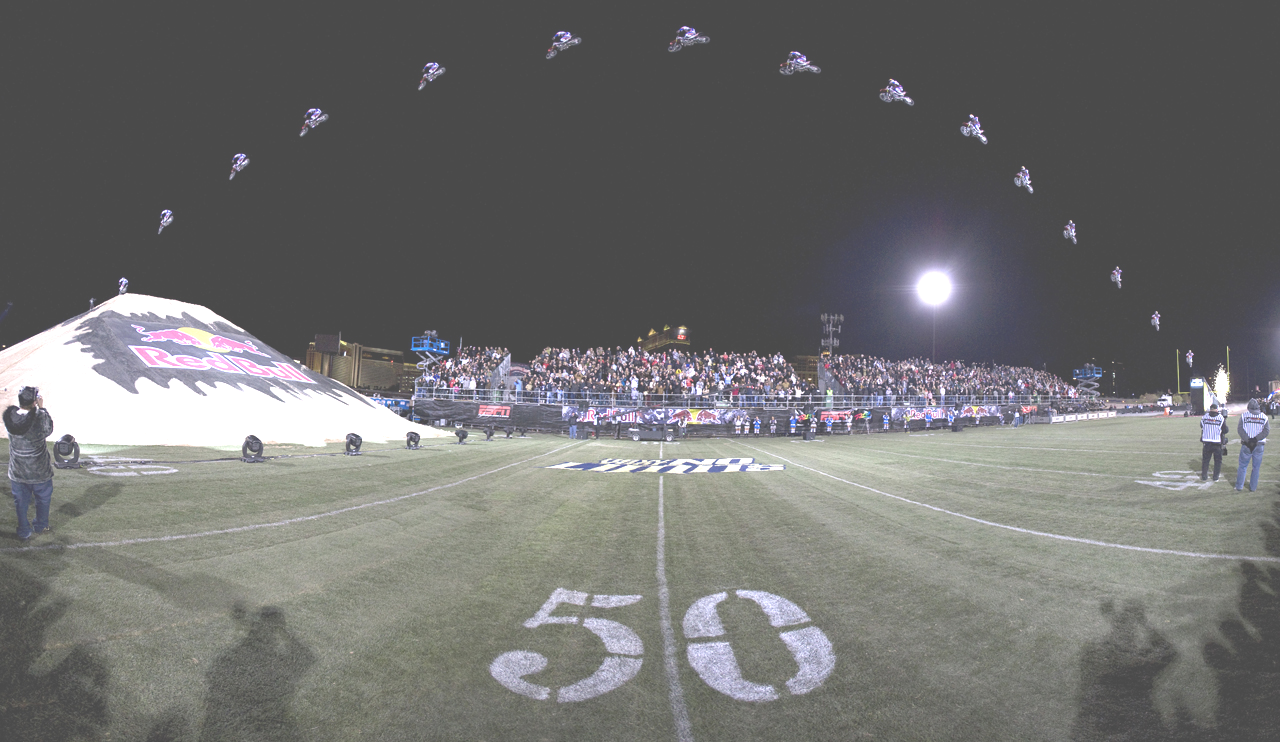
\includegraphics[width=.65\textwidth]{png/image1}
\end{center}


Le record du monde de saut en moto a été battu en 2008. L'australien Robbie Maddison a réussi un saut de
98,14 mètres (soit environ la longueur d'un terrain de football), et ceci deux fois de suite. L’événement a
eu lieu au Rio Hotel à Las Vegas pour célébrer la nouvelle année 2008.

\begin{minipage}[c]{.65\linewidth}
Pour réussir un tel saut, il est nécessaire d'avoir une suspension bien
réglée. On ne s'intéresse ici qu'au réglage de la suspension de la roue
arrière. Celle-ci est composée d'un amortisseur et d'un ressort . Le choix d'une raideur de ressort convenable permettra
d'éviter un ressenti de dureté lors de l'atterrissage. De la même
manière, un amortisseur correctement réglé permettra d'obtenir une
bonne stabilité.
\end{minipage}\hfill
\begin{minipage}[c]{.3\linewidth}

\begin{center}
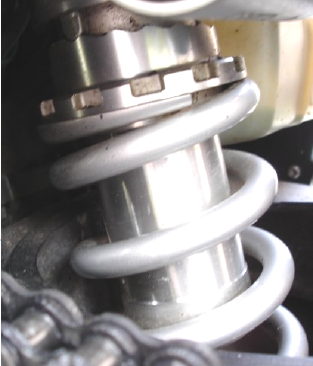
\includegraphics[width=.8\textwidth]{png/image2}
\end{center}
\end{minipage}

\begin{minipage}[c]{.5\linewidth}
On se propose de chercher un réglage théoriquement convenable de la
raideur et de l'amortisseur pour répondre à la contrainte suivante :
« Lors de l'atterrissage, pour éviter une chute, la moto doit atteindre
sa position d'équilibre le plus rapidement possible (0,3s) et être bien
amortie. »

On modélise la suspension de la moto par un système masse -- ressort -- amortisseur.

\end{minipage}\hfill
\begin{minipage}[c]{.45\linewidth}

\begin{center}
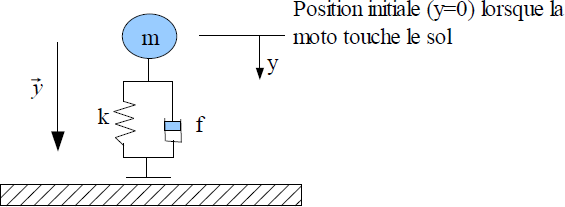
\includegraphics[width=.95\textwidth]{png/image3}
\end{center}
\end{minipage}


L'axe $\overrightarrow{y}$ est vertical descendant. On note $y(t)$ l'évolution de la position de la moto au cours du temps à
partir de la position initiale (lorsque la moto touche le sol).

La modélisation du choc lors de l'atterrissage revient à supposer que le système est soumis à un échelon de valeur $Mg$ (où $M$ est la somme de la masse de la moto et de la masse du conducteur et $g$ l'accélération de la pesanteur). Ce modèle
approximatif permet d'obtenir plusieurs valeurs caractéristiques.
}

L'équation différentielle, obtenue en écrivant le principe fondamental de la dynamique sur la masse $M$, est la suivante :
$$
\dfrac{d^2y(t)}{dt^2} + \dfrac{f}{M} \dfrac{dy(t)}{dt} + \dfrac{k}{M}y(t) = \dfrac{f(t)}{M}
$$

avec $f$ frottement visqueux, $k$ raideur du ressort, $M=100\;kg$ masse de l'ensemble \{moto+conducteur\}, $f(t)$
action exercée sur la masse.

\textbf{L'objectif de ce travail est donc de déterminer les paramètres $f$ et $k$ optimaux en analysant la réponse
temporelle $y(t)$.}


\section{Préliminaires}

%\subparagraph{} \textit{Exprimer $f(t)$ en fonction de $M$ et $g$ et en déduire $F(p)$.}

%\ifthenelse{\boolean{prof}}{
%\begin{corrige}

%\end{corrige}
%}{}

On note $f(t)=Mg\cdot u(t)$ avec $u(t)$ fonction de Heaviside. On a donc, $f(t)=Mg$ pour $t>0$. 

\subparagraph{}
\textit{Donner l'expression de $f(t)$ dans le domaine de Laplace.}


\ifthenelse{\boolean{prof}}{
\begin{corrige}
On a $\forall t>0$, $F(p)=\dfrac{Mg}{p}$.
\end{corrige}
}{}

\subparagraph{}
\textit{En utilisant l'expression obtenue pour $f(t)$, passer l'équation dans le domaine de Laplace
(on se place dans les conditions de Heaviside) et exprimer $Y(p)$ en fonction des données.}
\ifthenelse{\boolean{prof}}{
\begin{corrige}
Dans le domaine de Laplace, pour $t>0$, on a $
p^2Y(p) +\dfrac{f}{M}pY(p)+\dfrac{k}{M}Y(p)=\dfrac{g}{p}
$

On a donc :
$$
Y(p)=\dfrac{g}{p}\cdot\dfrac{1}{p^2+\dfrac{f}{M}p+\dfrac{k}{M}}
$$
\end{corrige}
}{}


\subparagraph{}
\textit{En utilisant le théorème de la valeur initiale, déterminer la position initiale.}

\ifthenelse{\boolean{prof}}{
\begin{corrige}
D'après le théorème de la valeur initiale, on a : 

$$
\lim\limits_{t\to 0} y(t)
= \lim\limits_{p\to +\infty} p\cdot Y(p)
= \lim\limits_{p\to +\infty} \dfrac{g}{p^2+\dfrac{f}{M}p+\dfrac{k}{M}}
= 0
$$
\end{corrige}
}{}

\subparagraph{}
\textit{En utilisant le théorème de la valeur finale, déterminer la position d'équilibre (position finale).}
\ifthenelse{\boolean{prof}}{
\begin{corrige}
D'après le théorème de la valeur finale, on a : 

$$
\lim\limits_{t\to +\infty} y(t)
= \lim\limits_{p\to 0} p\cdot Y(p)
= \lim\limits_{p\to 0} \dfrac{g}{p^2+\dfrac{f}{M}p+\dfrac{k}{M}}
= \dfrac{gM}{k}
$$
\end{corrige}
}{}


\subparagraph{}
\textit{Déterminer la pente de $y(t)$ à l'origine.}
\ifthenelse{\boolean{prof}}{
\begin{corrige}
La pente à l'origine correspond à la valeur initiale de la dérivée de $y(t)$ :
$$
\lim\limits_{t\to 0} \dfrac{dy(t)}{dt}
= \lim\limits_{p\to +\infty} p\cdot p\cdot  Y(p)
= \lim\limits_{p\to +\infty} \dfrac{g\cdot p}{p^2+\dfrac{f}{M}p+\dfrac{k}{M}}
= 0
$$

Il y a donc une asymptote horizontale à l'origine.


\end{corrige}
}{}


\subparagraph{}
\textit{Écrire $Y(p)$ (transformée de Laplace de $y(t)$) sous la forme 
$
Y(p)=\dfrac{g}{p\left( p^2+2 z \omega_0 p + \omega_0^2 \right)}
$.}
\textit{On exprimera $\omega_0$ et $z$ en fonction de $f$, $k$, $M$.}
\ifthenelse{\boolean{prof}}{
\begin{corrige}
$$
Y(p)=\dfrac{g}{p}\cdot\dfrac{1}{p^2+\dfrac{f}{M}p+\dfrac{k}{M}}
$$

On identifie donc les coefficients : $2z\omega_0=\dfrac{f}{M}$ et $\omega_0^2=\dfrac{k}{M}$.

On a donc $\omega_0=\sqrt{\dfrac{k}{M}}$ et $z=\dfrac{f}{2\omega_0 M}=\dfrac{f}{2\sqrt{\dfrac{k}{M}} M}=\dfrac{f}{2\sqrt{kM}}$.
\end{corrige}
}{}


Pour déterminer la réponse temporelle et étudier son allure, il est nécessaire de déterminer les racines du polynôme du second degré :
$$
D(p)=p^2+2z\omega_0 p + \omega_0^2
$$

\subparagraph{}
\textit{Déterminer la valeur de $z$ (nombre positif par définition) à partir de laquelle les racines sont réelles.}
\ifthenelse{\boolean{prof}}{
\begin{corrige}
Calculons le discriminant associé à $D(p)$ :
$$
\Delta = 4z^2\omega_0^2-4\omega_0^2=4\omega_0^2\left(z^2-1\right).
$$
Ainsi le $D(p)$ admet deux racines réelles lorsque $\Delta>0$ et que $z>1$.
\end{corrige}
}{}

\section{Cas de racines réelles}

On note $p_1=-\dfrac{1}{T_1}$ et $p_2=-\dfrac{1}{T_2}$ les deux racines réelles de $D(p)$, avec $T_1<T_2$.

\subparagraph{}
\textit{Donner l'expression de $T_1$ et $T_2$ en fonction de $\omega_0$ et $z$.}
\ifthenelse{\boolean{prof}}{
\begin{corrige}

En résolvant $D(p)=0$, on a :
$$
p_1=\dfrac{-2z\omega_0-\sqrt{\Delta}}{2} 
\quad 
p_2=\dfrac{-2z\omega_0+\sqrt{\Delta}}{2} 
\quad
\text{avec}\quad \sqrt{\Delta} = 2\omega_0 \sqrt{z^2-1}
$$

On a alors : 
$$
p_1=-z\omega_0-\omega_0 \sqrt{z^2-1}
\quad 
p_1=-z\omega_0+\omega_0 \sqrt{z^2-1}
$$

En conséquence, 
$$
T_1
=-\dfrac{1}{-z\omega_0-\omega_0 \sqrt{z^2-1}}
=\dfrac{1}{\omega_0\left(z+\sqrt{z^2-1}\right)}
\quad 
T_2
=-\dfrac{1}{-z\omega_0+\omega_0 \sqrt{z^2-1}}
=\dfrac{1}{\omega_0\left(z-\sqrt{z^2-1}\right)}
$$

\textit{Remarque : } On a bien $T_1<T_2$.
\end{corrige}
}{}


\subparagraph{}
\textit{Décomposer $Y(p)$ en éléments simples. On mettra $Y(p)$ sous la forme $Y(p)=\dfrac{A}{p}+\dfrac{B}{p-p_1}+\dfrac{C}{p-p_2}$. On exprimera $A$, $B$, $C$, $p_1$ et $p_2$ en fonction de $T_1$ et $T_2$.}
\ifthenelse{\boolean{prof}}{
\begin{corrige}
On pose :
$$
Y_1(p)=\dfrac{g}{p\left(p-p_1\right)\left(p-p_2\right)}
\quad
Y_2(p)=\dfrac{A}{p}+\dfrac{B}{p-p_1}+\dfrac{C}{p-p_2} 
\quad 
\text{avec}
\quad
Y(p)=Y_1(p)=Y_2(p)
$$

\begin{enumerate}
\item On multiplie $Y_1(p)$ et $Y_2(p)$ par $p$ puis on pose $p=0$. On a alors $A=\dfrac{g}{p_1p_2}$.
\item On multiplie $Y_1(p)$ et $Y_2(p)$ par $\left(p-p_1\right)$ puis on pose $p=p_1$. On a alors $B=\dfrac{g}{p_1\left(p_1-p_2\right)}$.
\item On multiplie $Y_1(p)$ et $Y_2(p)$ par $\left(p-p_2\right)$ puis on pose $p=p_2$. On a alors $C=\dfrac{g}{p_2\left(p_2-p_1\right)}$.
\end{enumerate}

On peut alors réexprimer $A$, $B$ et $C$ : 
\begin{itemize} 
\item $A=gT_1T_2$;
\item $B = \dfrac{g}{-\dfrac{1}{T_1}\left(-\dfrac{1}{T_1}+\dfrac{1}{T_2}\right)}=\dfrac{-gT_1}{\dfrac{T_1-T_2}{T_1T_2}}=\dfrac{gT_1^2T_2}{T_2-T_1}$
\item $C
=\dfrac{g}{-\dfrac{1}{T_2}\left(-\dfrac{1}{T_2}+\dfrac{1}{T_1}\right)}
=\dfrac{-gT_2}{\dfrac{T_2-T_1}{T_1T_2}}=\dfrac{gT_1T_2^2}{T_1-T_2}$
\end{itemize}

En conséquences,
$$
Y(p)=gT_1T_2 \left( \dfrac{1}{p}
+\dfrac{\dfrac{T_1}{T_2-T_1}}{p+\dfrac{1}{T_1}}
+\dfrac{\dfrac{T_2}{T_1-T_2}}{p+\dfrac{1}{T_2}}\right)
$$

\end{corrige}
}{}

\subparagraph{}
\textit{En déduire $y(t)$ en utilisant la transformée de Laplace inverse.}
\ifthenelse{\boolean{prof}}{
\begin{corrige}
Dans le domaine temporel on a donc, pour $t>0$ :
$$
y(t)=gT_1T_2 \left( 1
+\dfrac{T_1}{T_2-T_1} e^{-\dfrac{t}{T_1}}
+\dfrac{T_2}{T_1-T_2} e^{-\dfrac{t}{T_2}}
\right)
$$
\end{corrige}
}{}

\subparagraph{}
\textit{Tracer l'allure de $y(t)$.}
\ifthenelse{\boolean{prof}}{
\begin{corrige}

\end{corrige}
}{}



\subparagraph{}
\textit{\`A l'aide d'un logiciel adéquat (Libreoffice, Excel, gnuplot, ...), tracer l'évolution de $\dfrac{y(t)}{g / \omega_0^2}$.}


On tracera deux graphiques (contenant plusieurs courbes) mettant en évidence :
\begin{itemize}
\item l'influence de $z$ sur la réponse (en prenant $\omega_0=10\;rad/s$ et des valeurs de $z=\{1,1 ;1,5 ; 2, 3;5\}$);
\item l'influence de $\omega_0$ sur la réponse (en prenant $z=1,5$ et des valeurs de $\omega_0 = \{0,5;1;2;5;10\}\; rad/s$).
\end{itemize}

\ifthenelse{\boolean{prof}}{
\begin{corrige}
En utilisant les résultats de la question 8, on montre que $\omega_0^2=\dfrac{1}{T_1 \cdot T_2}$. En conséquence, 
$$
\dfrac{y(t)}{gT_1 T_2} = 
1
+\dfrac{T_1}{T_2-T_1} e^{-\dfrac{t}{T_1}}
+\dfrac{T_2}{T_1-T_2} e^{-\dfrac{t}{T_2}}
$$

En utilisant la librairie \textsf{matplotlib} de python on obtient les courbes suivantes

\end{corrige}
\begin{minipage}[c]{.47\linewidth}
\begin{center}
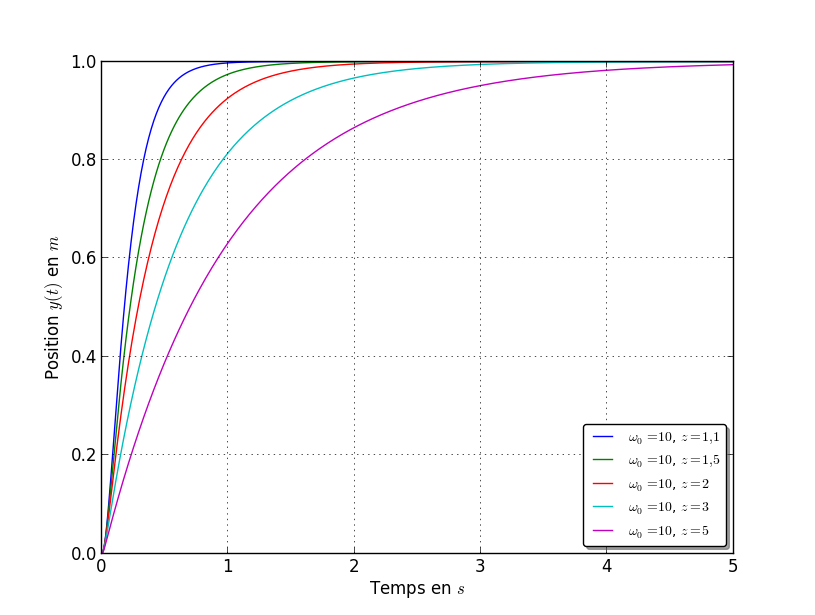
\includegraphics[width=\textwidth]{png/figure_1}
\end{center}
\end{minipage}\hfill
\begin{minipage}[c]{.47\linewidth}
\begin{center}
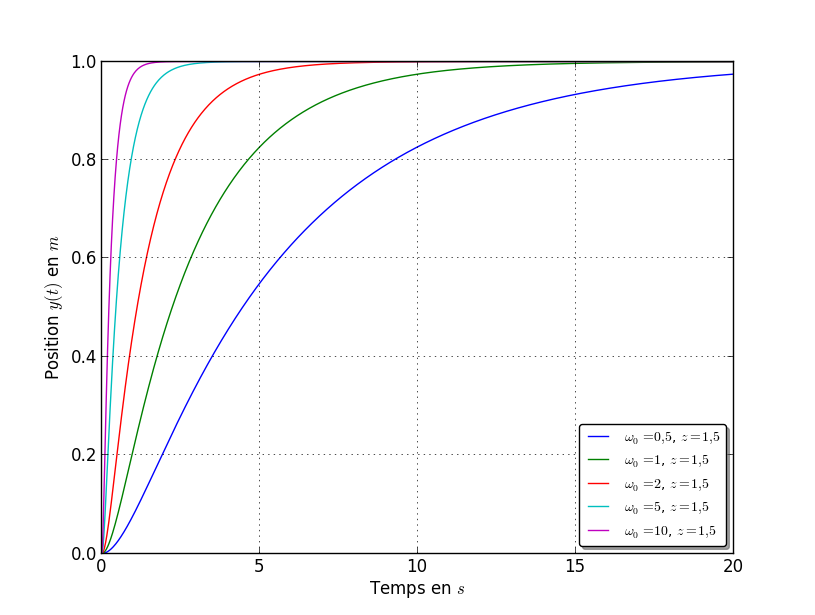
\includegraphics[width=\textwidth]{png/figure_2}
\end{center}
\end{minipage}
}{}


\subparagraph{}
\textit{Quelle valeur de $z$ permet d'obtenir un système rapide ?}
\ifthenelse{\boolean{prof}}{
\begin{corrige}
On peut observer que le temps de réponse à 5\% est le plus faible quand $z$ tend vers 1. 
\end{corrige}
}{}


\begin{minipage}[c]{.45\linewidth}

\subparagraph{Facultatif}
\textit{Sachant que l'allure de la réponse d'un système du premier ordre est la suivante. Donner les différences et les similitudes (on observera la pente à l'origine, la valeur asymptotique, l'allure,
les dépassements). Que dire si une des racines est très grande devant l'autre ?
($T_2 >> T_1$).}

\end{minipage}\hfill
\begin{minipage}[c]{.5\linewidth}
\begin{center}
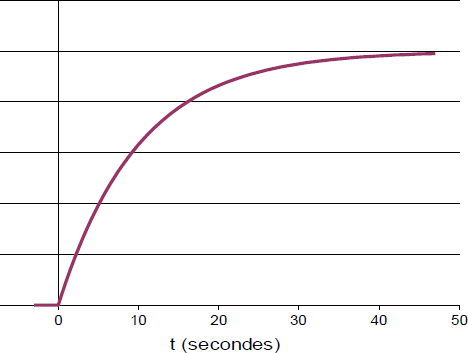
\includegraphics[width=.95\textwidth]{png/image4}
\end{center}
\end{minipage}

\ifthenelse{\boolean{prof}}{
\begin{corrige}

\begin{center}
\begin{tabular}{|l|l|l|}
\cline{2-3}
\multicolumn{1}{c|}{}& \textbf{Premier ordre} & \textbf{Second ordre} \\
\hline
Pente à l'origine & Non nulle & Nulle \\
\hline
Allure & \multicolumn{2}{c|}{Semblable} \\
\hline
Dépassement & \multicolumn{2}{c|}{Aucun} \\
\hline
\end{tabular}
\end{center}

\textit{Remarque :}  lorsque $\omega_0=10 rad/s$ on peut en déduire qu'une des racines devient négligeable devant l'autre. Le comportement de la sortie est donc proche du comportement d'un premier ordre. 
\end{corrige}
}{}

\end{document}

\section{Cas des racines complexes -- Facultatif}

Dans ces conditions, $Y(p)$ reste sous la forme :
$$
Y(p)=\dfrac{g}{p\left(p^2 + 2z\omega_0p +\omega_0^2\right)}
$$

\subparagraph{}
\textit{Décomposer $Y(p)$ en éléments simples.}
\ifthenelse{\boolean{prof}}{
\begin{corrige}
Sous cette forme, $Y(p)$ peut se décomposer ainsi :
$$
Y(p)=\dfrac{\alpha}{p}+\dfrac{\beta + \gamma p}{p^2 + 2z\omega_0p +\omega_0^2}
$$

En multipliant $Y(p)$ par $p$ et en posant $p=0$ on a immédiatement $\alpha = \dfrac{g}{\omega_0^2}$.

\textbf{Méthode 1 -- Valeurs particulières}

Calculons $Y(1)$ puis $Y(-1)$ :
$$
\dfrac{g}{1+2z\omega_0+\omega_0^2} = \dfrac{g}{\omega_0^2}  +\dfrac{\beta + \gamma }{1 + 2z\omega_0 +\omega_0^2}
\quad
\text{et}
\quad
-\dfrac{g}{1-2z\omega_0+\omega_0^2} = -\dfrac{g}{\omega_0^2}  +\dfrac{\beta - \gamma }{1 - 2z\omega_0 +\omega_0^2}
$$

On résout alors le système à deux équations deux inconnues.

\textbf{Méthode 2 -- Identification}

On a :
$$
Y(p)
=\dfrac{\alpha}{p}+\dfrac{\beta + \gamma p}{p^2 + 2z\omega_0p +\omega_0^2}
=\dfrac{\dfrac{g}{\omega_0^2}\left( p^2 + 2z\omega_0p +\omega_0^2 \right) + \beta p + \gamma p^2 }{p \cdot \left( p^2 + 2z\omega_0p +\omega_0^2\right)}
$$

$$
Y(p)
=\dfrac{\dfrac{g}{\omega_0^2} p^2 + 2z \dfrac{g}{\omega_0} p +g + \beta p + \gamma p^2 }{p \cdot \left( p^2 + 2z\omega_0p +\omega_0^2\right)}
=\dfrac{p^2\left( \dfrac{g}{\omega_0^2} + \gamma \right) + p\left( 2z \dfrac{g}{\omega_0}  + \beta \right) + g }{p \cdot \left( p^2 + 2z\omega_0p +\omega_0^2\right)}
$$
On a donc par identification avec la forme initiale de $Y(p)$ : 
$$
\left\{
\begin{array}{l}
 \dfrac{g}{\omega_0^2} + \gamma  = 0 \\
 2z \dfrac{g}{\omega_0}  + \beta = 0
\end{array}
\right.
\Longleftrightarrow
\left\{
\begin{array}{l}
\gamma = - \dfrac{g}{\omega_0^2} \\
\beta = -  2z \dfrac{g}{\omega_0}  
\end{array}
\right.
$$

\textbf{Méthode 3 -- Méthode des limites}

D'une part :
$$
\lim\limits_{p\to +\infty} p\cdot Y(p)=0
$$
D'autre part, 
$$
\lim\limits_{p\to +\infty} p\cdot Y(p)=\alpha + \gamma
$$

On a donc $\alpha + \gamma =0$.

Il reste donc à trouver une seconde équation par la méthode de votre choix. 

Au final, on a la forme de $Y(p)$ suivante : 
$$
Y(p)
=\dfrac{\dfrac{g}{\omega_0^2}}{p}+\dfrac{-  2z \dfrac{g}{\omega_0}  - \dfrac{g}{\omega_0^2} p}{p^2 + 2z\omega_0p +\omega_0^2}
=
\dfrac{g}{\omega_0^2} \left(
\dfrac{1}{p} 
-\dfrac{ 2z \omega_0  + p}{p^2 + 2z\omega_0p +\omega_0^2}
\right)
$$

\end{corrige}
}{}

\subparagraph{}
\textit{Modifier l'expression obtenue pour faire apparaître des formes caractéristiques du
tableau des transformées de Laplace. (On pourra poser $a=z\omega_0$ et $\omega_p^2=\omega_0^2\left(1-z^2 \right)$).}
\ifthenelse{\boolean{prof}}{
\begin{corrige}
Commençons par mettre $p^2 + 2z\omega_0p +\omega_0^2$ sous forme canonique : 
$$
p^2 + 2z\omega_0p +\omega_0^2 
= \left( p + z\omega_0\right)^2 -z^2\omega_0^2+\omega_0^2
= \left( p + a\right)^2 +\omega_p^2
$$

On a donc :
$$
Y(p)=\dfrac{g}{\omega_0^2} \left(
\dfrac{1}{p} 
-\dfrac{ 2a+ p}{\left( p + a\right)^2 +\omega_p^2}
\right)
=\dfrac{g}{\omega_0^2} \left(
\dfrac{1}{p} 
-\dfrac{ p+a}{\left( p + a\right)^2 +\omega_p^2}
-\dfrac{\omega_p}{\omega_p}\dfrac{ a}{\left( p + a\right)^2 +\omega_p^2}
\right)
$$

\end{corrige}
}{}




\subparagraph{}
\textit{Montrer alors que :}
$$
y(t)=K\left[
1-\dfrac{1}{\sqrt{1-z^2}}e^{-z\omega_0 t}\sin\left(
\omega_0\sqrt{1-z^2}t+\varphi
\right)
\right]
$$
\textit{avec $\varphi$ tel que $\cos\varphi=z$ et $\sin\varphi = \sqrt{1-z^2}$.}
\ifthenelse{\boolean{prof}}{
\begin{corrige}

Suite à la question précédente, dans le domaine temporel on a :
$$\forall t>0 \quad 
y(t)=
\dfrac{g}{\omega_0^2}
 \left(
1 
-e^{-at}\cos \left(\omega_p t\right)
-\dfrac{a}{\omega_p}e^{-at}\sin \left(\omega_p t\right)
\right)
$$

\begin{flushright}
\textbf{\textit{Calcul de trigonométrie à poursuivre...}}
\end{flushright}
%D'une part, 
%$$
%\dfrac{a}{\omega_p^2} = \dfrac{z}{\omega_0 \left(1-z^2\right)}
%$$
%
%D'autre part, montrons que $\dfrac{z}{\omega_0 \left(1-z^2\right)} = \dfrac{1}{\sqrt{1-z^2}}$
%
%
%On a :
%$$
%y(t)=
%\dfrac{g}{\omega_0^2}
% \left(
%1 
%-e^{-at}\left( \cos \left(\omega_p t\right)
%-\dfrac{a}{\omega_p^2} \sin \left(\omega_p t\right)
%\right)\right)
%$$

\end{corrige}
}{}


\subparagraph{}
\textit{Tracer à nouveau deux séries de courbes 
$\dfrac{y(t)}{g / \omega_0^2}$ mettant en évidence :
\begin{itemize}
\item l'influence de $z$ sur la réponse (en prenant $\omega_0=10\;rad /s$ et des valeurs de $z=\{0,1 ; 0,3 ; 0,5 ; 0,7 ; 0,9\}$);
\item l'influence de $\omega_0$ sur la réponse (en prenant $z= 0,5$ et des valeurs de $\omega_0=\{0,5 ; 1; 2,5; 10\}$).
\end{itemize}}
\ifthenelse{\boolean{prof}}{
\begin{minipage}[c]{.47\linewidth}
\begin{center}
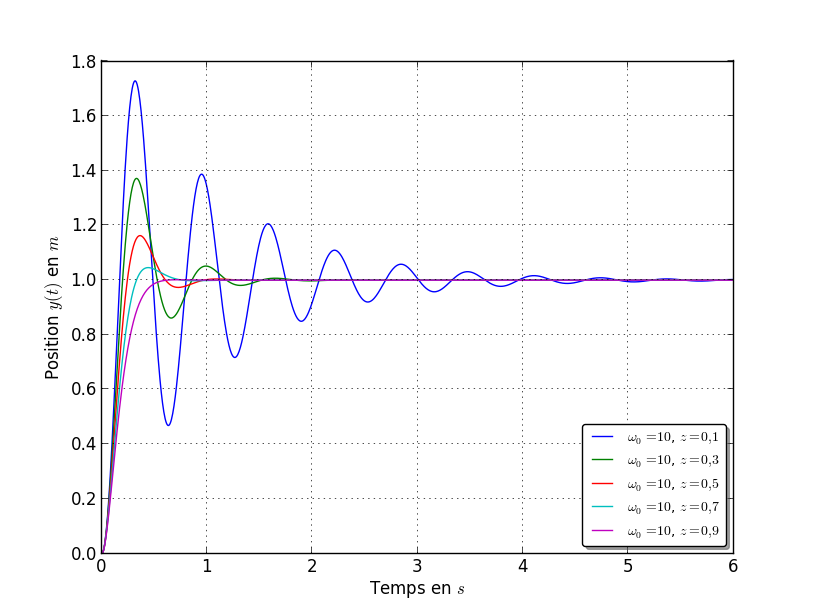
\includegraphics[width=\textwidth]{png/figure_3}
\end{center}
\end{minipage}\hfill
\begin{minipage}[c]{.47\linewidth}
\begin{center}
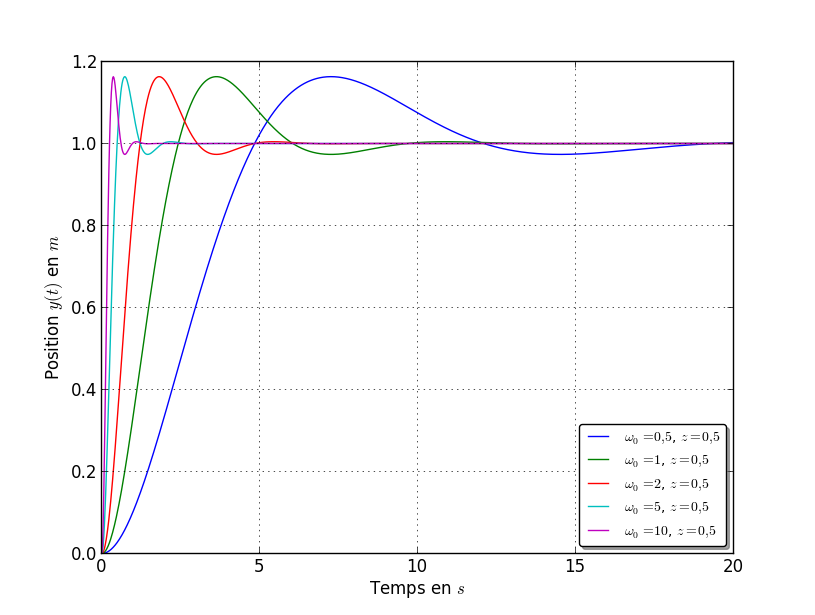
\includegraphics[width=\textwidth]{png/figure_4}
\end{center}
\end{minipage}
}{}

On voit apparaître sur ces courbes une pseudo-période $T$.

\subparagraph{}
\textit{Donner son expression à partir de $y(t)$.}
\ifthenelse{\boolean{prof}}{
\begin{corrige}
On a 
$$
y(t)=K\left[
1-\dfrac{1}{\sqrt{1-z^2}}e^{-z\omega_0 t}\sin\left(
\omega_0\sqrt{1-z^2}t+\varphi
\right)
\right]
$$
avec $\varphi$ tel que $\cos\varphi=z$ et $\sin\varphi = \sqrt{1-z^2}$.

La composante pseudo périodique vient de la composante $\sin\left(\omega_0\sqrt{1-z^2}t+\varphi \right)$. La période de de cette fonction est $T=\dfrac{2\pi}{\omega_0\sqrt{1-z^2}} $.
\end{corrige}
}{}

\subparagraph{}
\textit{Déterminer analytiquement les instants pour lesquels la dérivée de $y(t)$ est nulle. Ces
instants correspondent aux dépassements. (Vérifier le résultat obtenu sur les courbes tracées
précédemment.)}
\ifthenelse{\boolean{prof}}{
\begin{corrige}
Calculons la dérivée de $y(t)$ : 
$$
\dfrac{dy(t)}{dt}=
-\dfrac{g}{\omega_0^2\sqrt{1-z^2}}\left( 
-z\omega_0
e^{-z\omega_0 t}\sin\left( \omega_0\sqrt{1-z^2}t+\varphi \right)
+\omega_0\sqrt{1-z^2}
e^{-z\omega_0 t}\cos\left(
\omega_0\sqrt{1-z^2}t+\varphi
\right)
\right)
$$

$$
\dfrac{dy(t)}{dt}=
\dfrac{ge^{-z\omega_0 t}}{\omega_0\sqrt{1-z^2}} 
\left( z
\sin\left( \omega_0\sqrt{1-z^2}t+\varphi \right)
-\sqrt{1-z^2}
\cos\left(
\omega_0\sqrt{1-z^2}t+\varphi
\right)
\right)
$$
En posant $z=\cos\varphi$ et $\sqrt{1-z^2}=\sin\varphi$,
$$
\dfrac{dy(t)}{dt}=
\dfrac{ge^{-z\omega_0 t}}{\omega_0\sqrt{1-z^2}} 
\sin\left( \omega_0\sqrt{1-z^2}t\right)
$$

Ainsi, $\dfrac{dy(t)}{dt}=0$ lorsque $\omega_0\sqrt{1-z^2}t = k\pi$ soit $t=k\dfrac{\pi}{\omega_0\sqrt{1-z^2}}=\dfrac{kT}{2}$ avec $k\in\mathbb{N}$.

\end{corrige}
}{}

\subparagraph{}
\textit{Donner l'expression de ces dépassements.}
\ifthenelse{\boolean{prof}}{
\begin{corrige}
Pour avoir la valeur du $k$\ieme  dépassement, on commence par évaluer $y(t)$ en $\dfrac{kT}{2}$. 
On rappelle que $\sin(a+b)=\sin a \cos b + \sin b \cos a$ et que $\cos\varphi = z$.
Ainsi, 

$$
y\left(\dfrac{kT}{2}\right)=\dfrac{g}{\omega_0^2}\left[
1-\dfrac{1}{\sqrt{1-z^2}}e^{-z\omega_0 \dfrac{kT}{2}}\sin\left(
\omega_0\sqrt{1-z^2}\dfrac{kT}{2}+\varphi
\right)
\right]
$$

$$
y\left(\dfrac{kT}{2}\right)=\dfrac{g}{\omega_0^2}\left[
1-\dfrac{1}{\sqrt{1-z^2}}e^{-z\omega_0 k\dfrac{\pi}{\omega_0\sqrt{1-z^2}}}\sin\left(
\omega_0\sqrt{1-z^2}k\dfrac{\pi}{\omega_0\sqrt{1-z^2}}+\varphi
\right)
\right]
$$

$$
y\left(\dfrac{kT}{2}\right)
=\dfrac{g}{\omega_0^2}\left[
1-\dfrac{1}{\sqrt{1-z^2}}e^{\dfrac{-z k\pi}{\sqrt{1-z^2}}}\sin\left(
k \pi+\varphi \right)
\right]
=\dfrac{g}{\omega_0^2}\left[
1-\dfrac{1}{\sqrt{1-z^2}}e^{\dfrac{-z k\pi}{\sqrt{1-z^2}}}\cos\left(\varphi \right)
\right]
$$

$$
y\left(\dfrac{kT}{2}\right)
=\dfrac{g}{\omega_0^2}\left[
1-\dfrac{z}{\sqrt{1-z^2}}e^{\dfrac{-z k\pi}{\sqrt{1-z^2}}}
\right]
$$
\end{corrige}
}{}

\subparagraph{}
\textit{En faisant le rapport de l'écart entre les dépassements et la valeur asymptotique, et la valeur asymptotique ($D_{k\%} = \dfrac{s\left(t_k\right)-s_{\infty}}{s_{\infty}}$)
que remarque t-on ? Est-ce vérifié sur les courbes
obtenues ? }
\ifthenelse{\boolean{prof}}{
\begin{corrige}
\end{corrige}
}{}

\section{Réglages de la suspension -- Facultatif}

\subparagraph{}
\textit{\'A partir des différentes courbes obtenues, justifier graphiquement que la valeur de $z=0.7$
permette d'obtenir le système le plus rapide ? Calculer alors le premier taux de dépassement correspondant.}
\ifthenelse{\boolean{prof}}{
\begin{corrige}
\end{corrige}
}{}

\subparagraph{}
\textit{Pour cette valeur de $z$, on peut montrer que $t_{5\%}\cdot \omega_0 = \simeq 3$. Sachant qu'on souhaite
atteindre la position d'équilibre en $0,3\;s$, en déduire la valeur de $\omega_0$.}
\ifthenelse{\boolean{prof}}{
\begin{corrige}
\end{corrige}
}{}

\subparagraph{}
\textit{Tracer la courbe obtenue et vérifier que $t_{5\%}$ est correct et que la valeur obtenue pour le premier dépassement est également juste.}
\ifthenelse{\boolean{prof}}{
\begin{corrige}
\end{corrige}
}{}


\subparagraph{}
\textit{En conclusion, déterminer la valeur de $k$ et de $f$ permettant d'avoir les valeurs de $z$ et $\omega_0$ choisie précédemment.}
\ifthenelse{\boolean{prof}}{
\begin{corrige}
\end{corrige}
}{}


%\begin{center}
%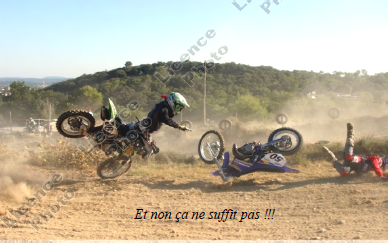
\includegraphics[width=.65\textwidth]{png/image5}
%\end{center}





\end{document}
